\begin{figure*}[!h]
  \centering
  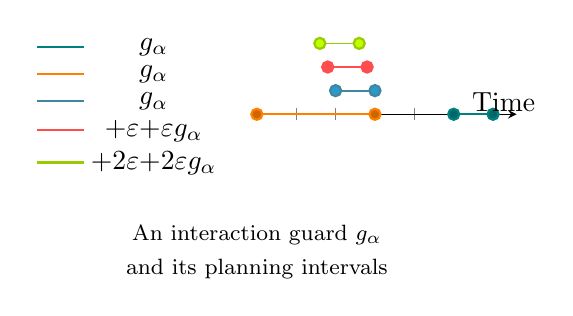
\begin{tikzpicture}[-]
  \begin{axis}[
   axis y line=none,
   y=0.3cm,
   x=1cm,
   xtick={15,15.5,16,...,18},
   restrict y to domain=1:5,
   axis lines=left,
   enlarge x limits=upper,
   cycle list name=exotic,
   scatter/classes={
   o={mark=*}
   },
   scatter,
   scatter src=explicit symbolic,
   every axis plot post/.style={mark=*,thick},
   xlabel=Time,
   x label style={at={(axis description cs:0.95,-0.1)},anchor=south},
   xticklabels={,,},
   legend style={
      draw=none,
      at={(-0.1,-1)},
      anchor=south east
  },
  legend image post style={mark=none}
  ]
  \addplot table [y expr=1,meta index=1, header=false] {
17.5 c
18 c
};\addlegendentry{$g_{\alpha}$}
    \addplot table [y expr=1,meta index=1, header=false] {
15 c
16.5 c
};\addlegendentry{$\backwardp{\hmin}{\hmx} g_{\alpha}$}
\addplot table [y expr=2,meta index=1, header=false] {
16.5 c
16 c
};\addlegendentry{$\backwardp{\hmin}{\hmin}g_{\alpha}$}
\addplot table [y expr=3,meta index=1, header=false] {
16.4 c
15.9 c
};\addlegendentry{$\backwardp{\hmin+\varepsilon}{\hmin+\varepsilon}g_{\alpha}$}
\addplot table [y expr=4,meta index=1, header=false] {
16.3 c
15.8 c
};\addlegendentry{$\backwardp{\hmin+2\varepsilon}{\hmin+2\varepsilon}g_{\alpha}$}
  \end{axis}
  \node (titile)[align=center,yshift=-1.75cm] {\footnotesize An interaction guard $g_{\alpha}$ \\ \footnotesize and its planning intervals};
\end{tikzpicture}
%  \caption{}
  %\captionsetup{justification=centering}
  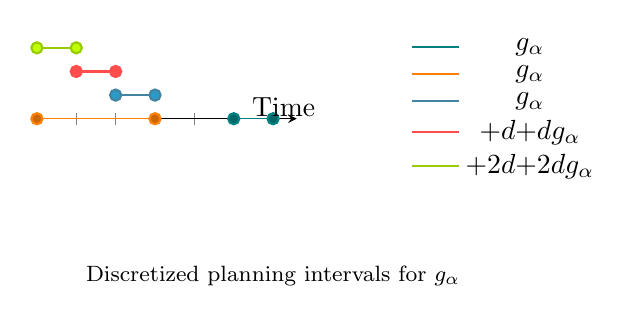
\begin{tikzpicture}[-]
  \begin{axis}[
   axis y line=none,
   y=0.3cm,
   x=1cm,  
   xtick={15,15.5,16,...,18},
   restrict y to domain=1:5,
   axis lines=left,
   enlarge x limits=upper,
   scatter/classes={
   o={mark=*,fill=white}
   },
   scatter,
   cycle list name=exotic,
   scatter src=explicit symbolic,
   every axis plot post/.style={mark=*,thick},
   xlabel=Time,
   x label style={at={(axis description cs:0.95,-0.1)},anchor=south},
   xticklabels={,,},
   legend style={
      draw=none,
      at={(2.2,-1)},
      anchor=south east
  },
  legend image post style={mark=none}
  ]
\addplot table [y expr=1,meta index=1, header=false] {
17.5 c
18 c
};\addlegendentry{$g_{\alpha}$}
\addplot table [y expr=1,meta index=1, header=false] {
15 c
16.5 c
};\addlegendentry{$\backwardp{\hmin}{\hmx} g_{\alpha}$}
\addplot table [y expr=2,meta index=1, header=false] {
16.5 c
16 c
};\addlegendentry{$\backwardp{\hmin}{\hmin}g_{\alpha}$}
\addplot table [y expr=3,meta index=1, header=false] {
16 c
15.5 c
};\addlegendentry{$\backwardp{\hmin+d}{\hmin+d}g_{\alpha}$}
\addplot table [y expr=4,meta index=1, header=false] {
15.5 c
15 c
};\addlegendentry{$\backwardp{\hmin+2d}{\hmin+2d}g_{\alpha}$}
  \end{axis}

  \node (titile)[align=center,yshift=-2cm,xshift=3cm] {\footnotesize Discretized planning intervals for $g_{\alpha}$};
  
\end{tikzpicture}
  %\caption{}
\caption{Discretizing Planning Horizons for Interaction}
\label{fig:disc}
\end{figure*}
